\zotelo{../thesis.bib}

\chapter{Higher order finite-difference schemes}
\label{app:finite-diff}

In this appendix we summarize the way to extend the finite difference scheme
described in chapter \ref{chap:pic} to higher orders. We assume symmetrically
staggered Yee grid as described in section \ref{sec:discretization}. In 1D the
position where the derivative is evaluated is staggered by half a cell with
respect to where the function value is evaluated (figure
\ref{fig:finite-diff-pos}).

\begin{figure}[h]
  \centering
  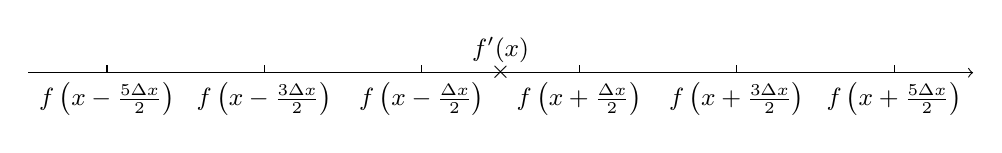
\begin{tikzpicture}[font=\small]
    \draw[->] (-6,0) -- node[midway,above] {$f'(x)$} (6,0);
    \node at (0,0) {$\times$};
    \draw (1,0) node[below] {$f\left(x + \frac{\Delta x}{2}\right)$} -- (1,0.1);
    \draw (3,0) node[below] {$f\left(x + \frac{3\Delta x}{2}\right)$} -- (3,0.1);
    \draw (5,0) node[below] {$f\left(x + \frac{5\Delta x}{2}\right)$} -- (5,0.1);
    \draw (-1,0) node[below] {$f\left(x - \frac{\Delta x}{2}\right)$} -- (-1,0.1);
    \draw (-3,0) node[below] {$f\left(x - \frac{3\Delta x}{2}\right)$} -- (-3,0.1);
    \draw (-5,0) node[below] {$f\left(x - \frac{5\Delta x}{2}\right)$} -- (-5,0.1);
  \end{tikzpicture}
  \caption{Positions where the function is evaluated and its derivative is
    evaluated in 1D.}
  \label{fig:finite-diff-pos}
\end{figure}

Now if we would like to find the 4th order accurate symmetric numerical
derivative, then we need to solve the following set of equations for
$f'(x)$:
\begin{align}
  \label{eq:4th-order-set}
  f \left( x - \frac{3\Delta x}{2} \right) &= f(x) - \frac{3\Delta x}{2}f'(x) + \frac{1}{2!}\left(\frac{3\Delta x}{2}\right)^2f''(x) - \frac{1}{3!}\left( \frac{3\Delta x}{2} \right)^{3}f'''(x) + O(\Delta x^4) \\
  f \left( x - \frac{\Delta x}{2} \right) &= f(x) - \frac{\Delta x}{2}f'(x) + \frac{1}{2!}\left(\frac{\Delta x}{2}\right)^2f''(x) - \frac{1}{3!}\left( \frac{\Delta x}{2} \right)^{3}f'''(x) + O(\Delta x^4) \\
  f \left( x + \frac{\Delta x}{2} \right) &= f(x) + \frac{\Delta x}{2}f'(x) + \frac{1}{2!}\left(\frac{\Delta x}{2}\right)^2f''(x) + \frac{1}{3!}\left( \frac{\Delta x}{2} \right)^{3}f'''(x) + O(\Delta x^4) \\
  f \left( x + \frac{3\Delta x}{2} \right) &= f(x) + \frac{3\Delta x}{2}f'(x) + \frac{1}{2!}\left(\frac{3\Delta x}{2}\right)^2f''(x) + \frac{1}{3!}\left( \frac{3\Delta x}{2} \right)^{3}f'''(x) + O(\Delta x^4)
\end{align}

The solution is (note that the 4th order term automatically cancels by symmetry,
the expression is accurate to 4th order in $\Delta x$):
\begin{equation}
  \label{eq:4th-order-sol}
  f'(x) = \frac{9}{8}\frac{f(x + \Delta x/2) - f(x - \Delta x / 2)}{\Delta x} - \frac{1}{24}\frac{f(x + 3\Delta x / 2) - f(x - 3\Delta x / 2)}{\Delta x} + O(\Delta x^5)
\end{equation}

One can repeat this procedure for $f'(x)$ up to any order in $\Delta x$. Table
\ref{tab:finite-diff} summarizes the coefficients for the results up to 6th
order accuracy.

\begin{table}[h]
  \centering
  \begin{tabular}{ccccccc}
    Order & $f(x - 5\Delta x/2)$ & $f(x - 3\Delta x / 2)$ & $f(x - \Delta x/2)$ & $f(x + \Delta x/2)$ & $f(x + 3\Delta x/2)$ & $f(x + 5\Delta x/2)$  \\ \hline
    2nd & 0 & 0 & -1 & 1 & 0 & 0 \\ \hline
    4th & 0 & 1/24 & -9/8 & 9/8 & -1/24 & 0 \\ \hline
    6th & -3/640 & 25/384 & -75/64 & 75/64 & -25/384 & 3/640 \\ \hline
  \end{tabular}
  \caption{Summary of 1D finite difference operator coefficients for evaluating $f'(x)$.}
  \label{tab:finite-diff}
\end{table}

Note that to achieve accuracy in terms of numerical truncation error, we
sacrifice locality: more and more adjacent grid points are used to evaluate the
local derivative. This has implications for communication, as the number of
guard cells for each boundary needs to be expanded to match the amount of
information that is needed to evaluate the derivative: for 2nd order derivative
we only need 1 guard cell, for 4th we need 2, and for 6th we need 3 layers of
guard cell, etc.

The number of guard cells is not the only problem however. When solving the
continuity equation \eqref{eq:continuity} the finite difference divergence
operator used must match the one used in updating the Maxwell equations. If we
use the above 4th order solution for evaluating curls in the Maxwell equations,
then we need to use the same 4th order operator for the continuity equation. To
my knowledge, there is no way to accomplish this using the Buneman current
deposition scheme (section \ref{sec:charge-cons-curr}), but it is possible using
the Esirkepov scheme. After one splits the continuity equation into components,
we now have:
\begin{equation}
  \label{eq:4th-order-esirkepov}
  \frac{9}{8}\left[ j_x(x+\Delta x/2) - j_x(x-\Delta x/2)\right] - \frac{1}{24}\left[ j_x(x + 3\Delta x/2) - j_x(x - 3\Delta x/2) \right] = -\frac{\Delta x}{\Delta t}\Delta \rho_x(x)
\end{equation}
Now it is not possible to solve these equations using a simple prefix sum, since
the current at different grid positions are coupled. This becomes a set of $N$
linear equations where $N$ equals the number of grid points in that direction.
It involves a band-diagonal matrix with alternating coefficients, which is known
to have unstable properties when solving numerically. However, instead of
solving for $j$ directly we can define $\Delta j_i = j_i - j_{i-1}$ where $i$
labels the grid points. Now the system of equations becomes
\begin{equation}
  \label{eq:4th-order-system}
  - \frac{1}{24}\Delta j_{i-1} + \frac{13}{12}\Delta j_i - \frac{1}{24}\Delta j_{i+1} = -\frac{\Delta x}{\Delta t}\Delta \rho_{i}
\end{equation}
which is a symmetric tri-diagonal system that is diagonally dominant. This kind
of systems has standard solvers and is generally numerically stable. After one
solves $\Delta j$ for every grid point, a prefix sum can be done similar to the
2nd order case to obtain $j$ for each cell. For 6th order finite difference, the
matrix becomes a band-diagonal system with 5 non-zero diagonals:
\begin{equation}
  \label{eq:6th-order-system}
  \frac{3}{640}\Delta j_{i-2} - \frac{29}{480}\Delta j_{i-1} + \frac{1067}{960}\Delta j_i - \frac{29}{480}\Delta j_{i+1} + \frac{3}{640}\Delta j_{i+2} = -\frac{\Delta x}{\Delta t}\Delta \rho_{i}
\end{equation}
which is also relatively simple to solve numerically.

Boundary condition is another problem. The main difficulty is the lack of
information across the boundary of the simulation domain, which means that the
typical symmetric finite difference cannot be used. A one-sided finite difference
scheme is required. Figure \ref{fig:1-sided-derivatives} shows two scenarios for
evaluating the one sided derivatives. One can find the correct coefficients by
writing down similar equations as \eqref{eq:4th-order-set} and the solutions are
given in tables \ref{tab:1-sided-a} and
\ref{tab:1-sided-b}. % TODO: finish this section

\begin{figure}[h]
  \centering
  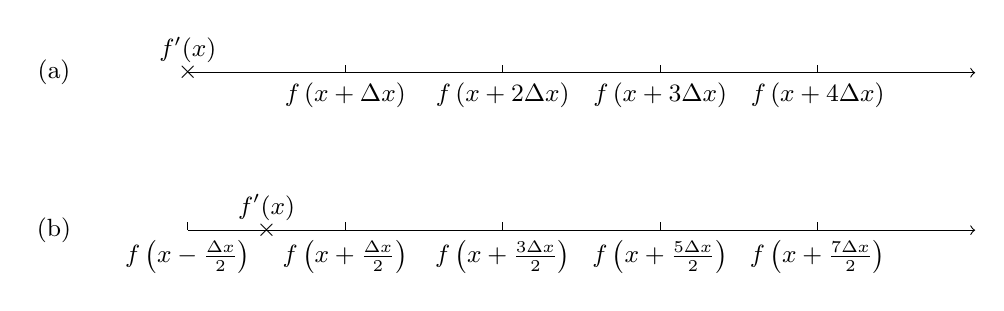
\begin{tikzpicture}[font=\small]
    \begin{scope}
      \node at (-1.7,0) {(a)};
      \draw[->] (0,0) node[above] {$f'(x)$} -- (10,0);
      \node at (0,0) {$\times$};
      \draw (2,0) node[below] {$f\left(x + \Delta x\right)$} -- (2,0.1);
      \draw (4,0) node[below] {$f\left(x + 2\Delta x\right)$} -- (4,0.1);
      \draw (6,0) node[below] {$f\left(x + 3\Delta x\right)$} -- (6,0.1);
      \draw (8,0) node[below] {$f\left(x + 4\Delta x\right)$} -- (8,0.1);
    \end{scope}
    \begin{scope}[yshift=-2cm]
      \node at (-1.7,0) {(b)};
      \draw[->] (0,0) -- (10,0);
      \draw (1,0) node {$\times$} -- (1,0) node[above] {$f'(x)$};
      \draw (0,0) node[below] {$f\left(x - \frac{\Delta x}{2}\right)$} -- (0,0.1);
      \draw (2,0) node[below] {$f\left(x + \frac{\Delta x}{2}\right)$} -- (2,0.1);
      \draw (4,0) node[below] {$f\left(x + \frac{3\Delta x}{2}\right)$} -- (4,0.1);
      \draw (6,0) node[below] {$f\left(x + \frac{5\Delta x}{2}\right)$} -- (6,0.1);
      \draw (8,0) node[below] {$f\left(x + \frac{7\Delta x}{2}\right)$} -- (8,0.1);
    \end{scope}
  \end{tikzpicture}
  \caption{Several scenarios for evaluating one-sided derivatives.}
  \label{fig:1-sided-derivatives}
\end{figure}

\begin{table}[h]
  \centering
  \begin{tabular}{cccccccc}
    Order & $f(x)$ & $f(x + \Delta x)$ & $f(x + 2\Delta x)$ & $f(x + 3\Delta x)$ & $f(x + 4\Delta x)$ & $f(x + 5\Delta x)$ & $f(x + 6\Delta x)$ \\ \hline
    2 & -3/2 & 2 & -1/2 & 0 & 0 & 0 & 0 \\ \hline
    4 & -25/12 & 4 & -3 & 4/3 & -1/4 & 0 & 0 \\ \hline
    6 & -147/60 & 6 & -15/2 & 20/3 & -15/4 & 6/5 & -1/6 \\ \hline
  \end{tabular}
  \caption[One-sided derivatives part 1]{One-sided derivatives for $f'(x)$ at the domain
    boundary. Scenario (a) in figure \ref{fig:1-sided-derivatives}}
  \label{tab:1-sided-a}
\end{table}

\begin{table}[h]
  \centering
  \begin{tabular}{cccccccc}
    Order & $f\left(x - \frac{\Delta x}{2}\right)$ & $f\left(x + \frac{\Delta x}{2}\right)$ & $f\left(x + \frac{3\Delta x}{2}\right)$ & $f\left(x + \frac{5\Delta x}{2}\right)$ & $f\left(x + \frac{7\Delta x}{2}\right)$ & $f\left(x + \frac{9\Delta x}{2}\right)$ & $f\left(x + \frac{11\Delta x}{2}\right)$ \\ \hline
    2 & -1 & 1 & 0 & 0 & 0 & 0 & 0 \\ \hline
    4 & -11/12 & 17/24 & 3/8 & -5/24 & 1/24 & 0 & 0 \\ \hline
    6 & -1627/1920 & 211/640 & 59/48 & -235/192 & 91/128 & -443/1920 & 31/960 \\ \hline
  \end{tabular}
  \caption[One-sided derivatives part 2]{One-sided derivatives for $f'(x)$ near the domain
    boundary. Scenario (b) in figure \ref{fig:1-sided-derivatives}}
  \label{tab:1-sided-b}
\end{table}



% Local Variables:
% TeX-master: "../thesis"
% zotero-collection: #("16" 0 2 (name "Thesis"))
% End: